% 
%  chapter2.tex
%  ThesisISEL
%  
%  Created by Matilde Pós-de-Mina Pato on 2012/10/09.
%
\chapter{Related Work}
\label{cha:related_work}

The following chapter showcases related work relevant to this thesis project.

We’ll start by clearly defining a learning disability (Section \ref{section:learningdisabilityexplanation}), which will help us design strategies to overcome these challenges. To better tailor the project to our intended users, we’ll dive deep into research on each type of learning disability (Section \ref{sec:overcomingLds}).

After that, we will look into existing solutions on the market that can inform and enhance the development of this project (Section \ref{sec:gamesforld}).


% ================
% = Introduction =
% ================
\section{Learning Disabilities}
\label{section:learningdisabilityexplanation}
A \gls{ld} is a variation of neurological conditions that can affect the capacity of a person to process, understand and remember information or specific learning abilities, even when a person’s intelligence is normal and learning opportunities are suitable.

These conditions can affect abilities such as reading, mathematics, reasoning, logic, visual and auditive comprehension, memory, and information organization. The common types of learning disabilities include dyslexia and dyscalculia \cite{NINDSLearningDisabilities}.

%, and ADHD (Attention deficit and hyperactive disorder).

The main causes of learning disabilities are not fully understood, but it’s believed that genealogical, neurobiological, and environmental factors can be a root cause. It’s important to highlight that learning disabilities aren’t caused by lack of effort, motivation, or intelligence \cite{UniversityWashingtonLearningDisabilities}.

The diagnostic and treatment of learning disabilities can include a combination of educational interventions, behavioural therapies and medication, depending on the seriousness and the individual needs of each affected people. It is known that the practice of educational games can also overcome learning disabilities \cite{NINDSLearningDisabilities}.

\section{Overcoming Learning Disabilities}
\label{sec:overcomingLds}
	% (Apresentar as definições das dificuldades de aprendizagem)
	% (Colocar as referências para a bibliografia da área da psicologia)
	% (Explicar as razões pelas quais os jogos são adequados para combater
	% as dificuldades de aprendizagem)

Children with learning disabilities face unique challenges both in their educational and social life. The use of interactive technology, specifically games, has shown great promise in helping these kids to deal with situations by providing an engaging learning experience specifically tailored for them. In this section, the state-of-the-art about the series of mini-games for supporting children with learning disabilities is addressed.

\textbf{Game Based Learning} \acrshort{gbl} has emerged as an innovative approach to address the specific needs of children with \gls{ld}'s. This technique utilizes the power of games to define and support learning outcomes. This is a great way to help them learn due to the fact that games are already a big part in most of the children's playtime. The evolution of technology has provided lots of different ways people can play games and we often see children playing more in their laptop, tablet and even their smartphones. A \acrshort{gbl} environment achieves these learning outcomes through educational games that have elements such as engagement, rewards, and healthy competition, making people stay motivated while learning \cite{gblProsCons}.
% https://www.edutopia.org/topic/game-based-learning/
% https://www.prodigygame.com/main-en/blog/game-based-learning/
% https://files.eric.ed.gov/fulltext/EJ1090277.pdf


Some important points should be addressed when designing a product like this. First of all, understanding the nature of \acrshort{ld}'s is crucial. \gls{ld}'s encompass a range of conditions that include Dyslexia, Dyscalculia, \acrfull{lpd}, Non-Verbal Learning Disabilities, Dysgraphia, Auditory Processing Disorder, and Visual Motor Deficit.

% Explain each learning disabilities
In order to properly develop these mini-games we should have in mind the characteristics of these disabilities. This way, some research was done so that we can better understand each \acrshort{ld}. For each one, we created a ``User Profile`` that contains the most likely Problems, Goals, Misconceptions, Needs, and Psychographics.
\newpage
\subsection{Dyslexia}
Dyslexia is a common learning disability that affects reading and language processing skills. Children with dyslexia often struggle with various aspects of reading, including decoding, spelling, reading comprehension, and phonological memory. Understanding the user profile associated with dyslexia can guide the development of effective mini-games to address the specific goals, psychographics, problems, facts, and needs of children with this learning disability.

\paragraph{\textbf{Goals}}
\begin{itemize}
    \item \textbf{Help children understand their disability}: The mini-games aim to provide children with a clear understanding of dyslexia, its effects on reading, and how it does not define their intelligence or potential.
    \item \textbf{Foster empathy and self-acceptance}: By creating an environment that encourages self-compassion and understanding, the mini-games aim to instill a sense of empathy within children towards themselves and others facing similar challenges.
    \item \textbf{Promote improvement through appropriate support}: The mini-games strive to demonstrate how with the right help and a supportive environment, children with dyslexia can make significant improvements in their reading abilities.
    \item \textbf{Cultivate a sense of achievement}: Recognizing and celebrating every milestone and achievement, no matter how small, is a key objective of the mini-games.
    \item \textbf{Normalize failure and embrace mistakes}: The mini-games aim to shift the perception of failure by illustrating that mistakes are an inherent part of the learning process and can lead to positive growth.
\end{itemize}

\paragraph{\textbf{Psycographics}}
\begin{itemize}
    \item \textbf{Low self-esteem}: Dyslexia can negatively impact self-esteem due to difficulties experienced in reading and academic settings. \cite{dyslexiaUnderstanding}
    \item \textbf{High persistence}: Children with dyslexia often exhibit determination and persistence in overcoming challenges related to reading. \cite{dyslexiaStatistics}
    \item \textbf{Medium-low sociability}: Children with dyslexia may exhibit varying levels of sociability, often preferring smaller social groups or activities that do not heavily rely on reading. \cite{dyslexiaClinic}
    \item \textbf{High self-consciousness}: Dyslexia can make children self-conscious about their reading abilities, leading to heightened self-awareness in educational settings.
    \item \textbf{Low laziness}: Despite the challenges they face, children with dyslexia typically demonstrate a strong work ethic and a drive to overcome difficulties. \cite{dyslexiaStatistics}
\end{itemize}

\paragraph{\textbf{Problems}}
\begin{itemize}
    \item \textbf{Reading}: Difficulties in accurately and fluently recognizing and decoding words. \cite{dyslexiaCharAndSigns}
    \item \textbf{Reading Aloud}: Challenges in pronouncing words correctly and maintaining fluency while reading aloud. \cite{dyslexiaCharAndSigns}
    \item \textbf{Spelling}: Struggles with accurate spelling due to difficulties in connecting sounds to letters and understanding spelling patterns. \cite{dyslexiaCharAndSigns}
    \item \textbf{Reading Comprehension}: Difficulties in understanding and deriving meaning from written text, impacting overall comprehension skills.\cite{dyslexiaCharAndSigns}
    \item \textbf{Phonological Memory}: Challenges in remembering and manipulating speech sounds, affecting phonemic awareness and decoding skills. \cite{dyslexiaCharAndSigns}
\end{itemize}

\paragraph{\textbf{Facts}}
\begin{itemize}
    \item Dyslexia does not prevent individuals from learning how to read. \cite{dyslexiaCharAndSigns}
    \item Intelligence is not a determining factor in the presence of dyslexia. \cite{dyslexiaStatistics}
    \item Dyslexia affects both boys and girls. \cite{dyslexiaCharAndSigns}
    \item Dyslexia is a lifelong learning disability, but individuals can make significant progress with appropriate interventions and support. \cite{dyslexiaCharAndSigns}
    \item Dyslexia primarily affects reading, not oral language skills. \cite{dyslexiaCharAndSigns}
    \item Reversing letters or words is not exclusive to dyslexia. \cite{dyslexiaCharAndSigns}
    \item Dyslexia is a relatively common learning disability.
    \item Dyslexia is not caused by a lack of effort or motivation to learn how to read.
\end{itemize}

\paragraph{\textbf{Needs}}
\begin{itemize}
    \item \textbf{Multi-sensory instruction in decoding skills}: Children with dyslexia benefit from instructional approaches that engage multiple senses simultaneously. This approach typically involves integrating visual, auditory, and kinesthetic modalities to reinforce letter-sound relationships and improve reading accuracy. For example, a mini-game could present letters or words visually while simultaneously providing auditory feedback or encouraging physical manipulation of letter tiles. \cite{dyslexiaUnderstanding}
    \item \textbf{Repetition and review of skills}: Dyslexic learners require ample opportunities for practice and reinforcement of decoding skills. Repetition helps solidify their understanding of letter-sound associations, spelling patterns, and reading strategies. Mini-games can incorporate repeated exposure to target skills through varied and engaging activities, allowing children to reinforce their learning in an interactive and enjoyable manner. \cite{dyslexiaUnderstanding}
    \item \textbf{Small group or individual instruction}: Dyslexia-specific instruction often benefits from personalized attention in small group settings or one-on-one instruction. Mini-games can be designed to accommodate different group sizes, allowing for targeted interventions and tailored support. Providing individualized feedback and adaptive features within the games can further enhance the effectiveness of small group or individual instruction. \cite{dyslexiaUnderstanding}
    \item \textbf{Teaching decoding skills}: Dyslexic children often struggle with decoding, the process of translating written words into spoken language. Mini-games can focus on teaching and reinforcing decoding skills by incorporating activities that require the identification and blending of letter sounds, syllables, or whole words. Interactive feedback and scaffolding mechanisms can guide children through the decoding process, promoting accuracy and fluency. \cite{dyslexiaUnderstanding}
    \item \textbf{Drilling sight words}: Sight words, also known as high-frequency words, are common words that dyslexic learners encounter frequently but do not follow regular phonetic patterns. Mini-games can include drills and practice exercises that specifically target sight words. By presenting these words repeatedly in engaging formats, such as word recognition games or word-building puzzles, dyslexic learners can improve their automatic recognition and reading fluency. \cite{dyslexiaUnderstanding}
    \item \textbf{Teaching comprehension strategies to help derive meaning from text}: Reading comprehension is a significant challenge for individuals with dyslexia. Mini-games can incorporate activities that teach and reinforce comprehension strategies, such as identifying main ideas, making inferences, summarizing information, and visualizing text. By practicing these strategies within interactive game contexts, children with dyslexia can develop stronger comprehension skills and derive meaning from what they read. \cite{dyslexiaUnderstanding}
\end{itemize}

% https://www.fcps.edu/academics/academic-overview/special-education-instruction/high-incidence-disabilities-team-k-12-2
% https://www.mayoclinic.org/diseases-conditions/dyslexia/symptoms-causes/syc-20353552
% https://childmind.org/article/understanding-dyslexia/
% https://www.crossrivertherapy.com/research/dyslexia-statistics
% Add image

% \begin{itemize}
%     \item \textbf{Goals}
%     \begin{itemize}
%         \item \textbf{Help children understand their disability}: The mini-games aim to provide children with a clear understanding of dyslexia, its effects on reading, and how it does not define their intelligence or potential.
%         \item \textbf{Foster empathy and self-acceptance}: By creating an environment that encourages self-compassion and understanding, the mini-games aim to instill a sense of empathy within children towards themselves and others facing similar challenges.
%         \item \textbf{Promote improvement through appropriate support}: The mini-games strive to demonstrate how with the right help and a supportive environment, children with dyslexia can make significant improvements in their reading abilities.
%         \item \textbf{Cultivate a sense of achievement}: Recognizing and celebrating every milestone and achievement, no matter how small, is a key objective of the mini-games.
%         \item \textbf{Normalize failure and embrace mistakes}: The mini-games aim to shift the perception of failure by illustrating that mistakes are an inherent part of the learning process and can lead to positive growth.
%     \end{itemize}
%     \item \textbf{Psycographics}
%     \begin{itemize}
%         \item \textbf{High persistence}: Children with dyslexia often exhibit determination and persistence in overcoming challenges related to reading.
%         \item \textbf{Low self-esteem}: Dyslexia can negatively impact self-esteem due to difficulties experienced in reading and academic settings.
%         \item \textbf{Medium-low sociability}: Children with dyslexia may exhibit varying levels of sociability, often preferring smaller social groups or activities that do not heavily rely on reading.
%         \item \textbf{High self-consciousness}: Dyslexia can make children self-conscious about their reading abilities, leading to heightened self-awareness in educational settings.
%         \item \textbf{Low laziness}: Despite the challenges they face, children with dyslexia typically demon   strate a strong work ethic and a drive to overcome difficulties.
%     \end{itemize}
%     \item \textbf{Problems}
%     \begin{itemize}
%         \item \textbf{Reading}: Difficulties in accurately and fluently recognizing and decoding words.
%         \item \textbf{Reading Aloud}: Challenges in pronouncing words correctly and maintaining fluency while reading aloud.
%         \item \textbf{Spelling}: Struggles with accurate spelling due to difficulties in connecting sounds to letters and understanding spelling patterns.
%         \item \textbf{Reading Comprehension}: Difficulties in understanding and deriving meaning from written text, impacting overall comprehension skills.
%         \item \textbf{Phonological Memory}: Challenges in remembering and manipulating speech sounds, affecting phonemic awareness and decoding skills.
%     \end{itemize}
%     \item \textbf{Misconceptions}
%     \begin{itemize}
%         \item Dyslexia does not prevent individuals from learning how to read.
%         \item Intelligence is not a determining factor in the presence of dyslexia.
%         \item Dyslexia affects both boys and girls.
%         \item Dyslexia is a lifelong learning disability, but individuals can make significant progress with appropriate interventions and support.
%         \item Dyslexia primarily affects reading, not oral language skills.
%         \item Reversing letters or words is not exclusive to dyslexia.
%         \item Dyslexia is a relatively common learning disability.
%         \item Dyslexia is not caused by a lack of effort or motivation to learn how to read.
%     \end{itemize}
%     \item \textbf{Needs}
%     \begin{itemize}
%         \item \textbf{Multi-sensory instruction in decoding skills}: Children with dyslexia benefit from instructional approaches that engage multiple senses simultaneously. This approach typically involves integrating visual, auditory, and kinesthetic modalities to reinforce letter-sound relationships and improve reading accuracy. For example, a mini-game could present letters or words visually while simultaneously providing auditory feedback or encouraging physical manipulation of letter tiles.
%         \item \textbf{Repetition and review of skills}: Dyslexic learners require ample opportunities for practice and reinforcement of decoding skills. Repetition helps solidify their understanding of letter-sound associations, spelling patterns, and reading strategies. Mini-games can incorporate repeated exposure to target skills through varied and engaging activities, allowing children to reinforce their learning in an interactive and enjoyable manner.
%         \item \textbf{Small group or individual instruction}: Dyslexia-specific instruction often benefits from personalized attention in small group settings or one-on-one instruction. Mini-games can be designed to accommodate different group sizes, allowing for targeted interventions and tailored support. Providing individualized feedback and adaptive features within the games can further enhance the effectiveness of small group or individual instruction.
%         \item \textbf{Teaching decoding skills}: Dyslexic children often struggle with decoding, the process of translating written words into spoken language. Mini-games can focus on teaching and reinforcing decoding skills by incorporating activities that require the identification and blending of letter sounds, syllables, or whole words. Interactive feedback and scaffolding mechanisms can guide children through the decoding process, promoting accuracy and fluency.
%         \item \textbf{Drilling sight words}: Sight words, also known as high-frequency words, are common words that dyslexic learners encounter frequently but do not follow regular phonetic patterns. Mini-games can include drills and practice exercises that specifically target sight words. By presenting these words repeatedly in engaging formats, such as word recognition games or word-building puzzles, dyslexic learners can improve their automatic recognition and reading fluency.
%         \item \textbf{Teaching comprehension strategies to help derive meaning from text}: Reading comprehension is a significant challenge for individuals with dyslexia. Mini-games can incorporate activities that teach and reinforce comprehension strategies, such as identifying main ideas, making inferences, summarizing information, and visualizing text. By practicing these strategies within interactive game contexts, children with dyslexia can develop stronger comprehension skills and derive meaning from what they read.
%     \end{itemize}
% \end{itemize}

\subsection{Language Processing Disorder}
\gls{lpd} are neurodevelopmental conditions that hinder a child’s ability to understand and use spoken language effectively. Individuals with \gls{lpd} may face challenges with both understanding others and expressing themselves verbally, which can impact their social interactions, academic performance, and overall communication skills. Developing interventions tailored to children with \gls{lpd} requires a deep understanding of their unique profiles. This means identifying their specific goals, psychographics, problems, characteristics, and needs related to language processing. Figure \ref{fig:lpdUserProfile} depicts the \gls{lpd} user profile.

\begin{figure}[H]
    \centering
    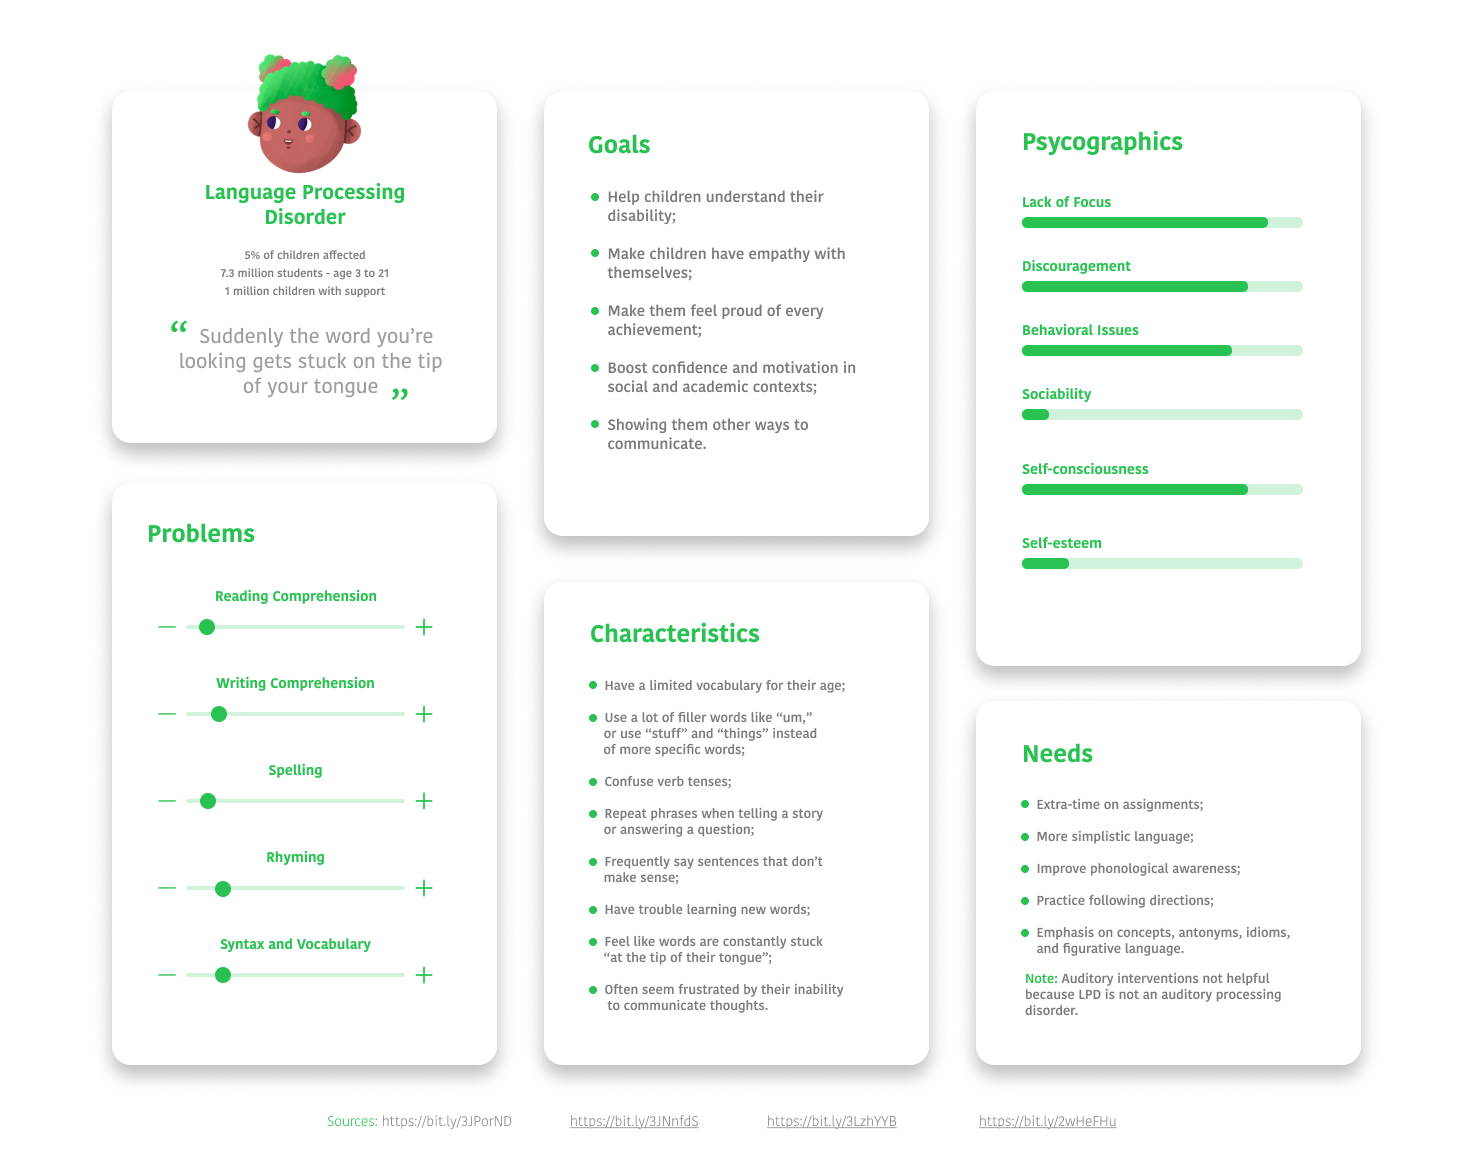
\includegraphics[width=1\linewidth]{Chapters/figma/Language Processing Disorder.png}
    \caption{Language Processing Disorder User Profile}
    \label{fig:lpdUserProfile}
\end{figure}

\paragraph{Goals}
\begin{itemize}
    \item \textbf{Help children understand their disability}: The mini-games aim to provide children with a clear understanding of Language Processing Disorder, its impact on their language skills, and how it does not define their intelligence or potential.
    \item \textbf{Foster empathy and self-acceptance}: By creating an environment that encourages self-compassion and understanding, the mini-games aim to instill a sense of empathy within children towards themselves and others facing similar challenges.
    \item \textbf{Foster pride in achievements}: Recognizing and celebrating every accomplishment, no matter how small, is a key objective of the mini-games.
    \item \textbf{Boost confidence and motivation in social and academic context}: The mini-games aim to enhance children's confidence and motivation to communicate effectively in social and academic settings.
    \item \textbf{Explore alternative communication methods}: The mini-games can introduce children to different ways of communication, such as visual aids, gestures, or assistive technologies, to overcome challenges related with language processing.
\end{itemize}

\paragraph{Psycographics}
\begin{itemize}
    \item \textbf{Low self-esteem}: Struggles with language processing can negatively impact children's self-esteem, making it important to design mini-games that foster a sense of accomplishment and build confidence \cite{vanderbilt}.
    \item \textbf{Low sociability}: Due to communication challenges, children may show a preference for limited social interactions or struggle with initiating and maintaining conversations \cite{greatspeech}.
    \item \textbf{High lack of focus}: Children with \gls{lpd} may struggle with keeping attention and concentration, making it important to design engaging and interactive mini-games \cite{vanderbilt}.
    \item \textbf{High discouragement}: Difficulties in language processing can lead to frustration and discouragement in academic and social contexts.
    \item \textbf{High behavioral issues}: Children with Language Processing Disorder may exhibit behavioral challenges stemming from their communication difficulties \cite{vanderbilt}.
    \item \textbf{High self-consciousness}: Language difficulties can make children self-conscious about their communication abilities, leading to heightened self-awareness in social and educational settings \cite{additude}.
\end{itemize}

\paragraph{Problems}
\begin{itemize}
    \item \textbf{Reading and Writing Comprehension}: Difficulties in understanding and extracting meaning from written text and expressing thoughts in writing \cite{vanderbilt}.
    \item \textbf{Spelling}: Challenges in accurately spelling words due to difficulties in phonemic awareness and sound-letter correspondence \cite{vanderbilt}.
    \item \textbf{Rhyming}: Difficulty recognizing and generating rhyming words, impacting phonological awareness \cite{vanderbilt}.
    \item \textbf{Syntax and Vocabulary}: Challenges with understanding and using grammatical rules and acquiring and retaining a wide range of vocabulary \cite{additude}.
\end{itemize}

\paragraph{Characteristics}
\begin{itemize}
    \item \textbf{Limited vocabulary for their age}: They may have a smaller repertoire of words compared to their peers \cite{additude}.
    \item \textbf{Use of filler words and vague language}: They may rely on filler words like ''hum'' or use general terms like ''stuff'' and ''things'' instead of specific words \cite{additude}.
    \item \textbf{Confusion with verb tenses}: Difficulties in using and understanding appropriate verb tenses \cite{greatspeech}.
    \item \textbf{Repetition of phrases}: They may repeat phrases when telling stories or answering questions \cite{additude}.
    \item \textbf{Incoherent sentences}: Frequent production of sentences that do not make sense or lack cohesion \cite{additude}.
    \item \textbf{Trouble learning new words}: Challenges in acquiring and retaining new vocabulary \cite{additude}.
    \item \textbf{Tip-of-the-tongue phenomenon}: Feelings of frustration when they cannot retrieve specific words or express their thoughts \cite{additude}.
\end{itemize}

\paragraph{Needs}
\begin{itemize}
    \item \textbf{Extra time on assignments}: Providing additional time for completing tasks and assignments to accommodate the slower processing speed \cite{vanderbilt}.
    \item \textbf{Simplified language}: Using clear and concise language that is appropriate for the children's understanding level and to avoid complex sentence structures \cite{additude}.
    \item \textbf{Improving phonological awareness}: Incorporating activities in the mini-games that focus on recognizing and manipulating sounds within words, such as rhyming, segmenting, and blending \cite{vanderbilt}.
    \item \textbf{Practice following directions}: Designing mini-games that involve following sequential instructions to improve understanding and processing of spoken language \cite{vanderbilt}.
    \item \textbf{Emphasis on concepts, antonyms, idioms, and figurative language}: Including activities that target understanding and using abstract language concepts, such as opposites, idiomatic expressions, and figurative language, to expand their language skills \cite{vanderbilt}.
\end{itemize}


\subsection{Dyscalculia}

Dyscalculia is a learning disorder that primarily affects a child's ability to understand and work with numbers. Individuals with dyscalculia often encounter challenges in basic arithmetic operations, number sense, and mathematical reasoning. To develop effective interventions for children with dyscalculia, it is crucial to understand their unique user profile. This includes identifying their specific goals, psychographics, problems, characteristics and needs related to mathematical learning. Figure \ref{fig:dyscalculiaUserProfile} depicts the Dyscalculia user profile.

\begin{figure}[H]
    \centering
    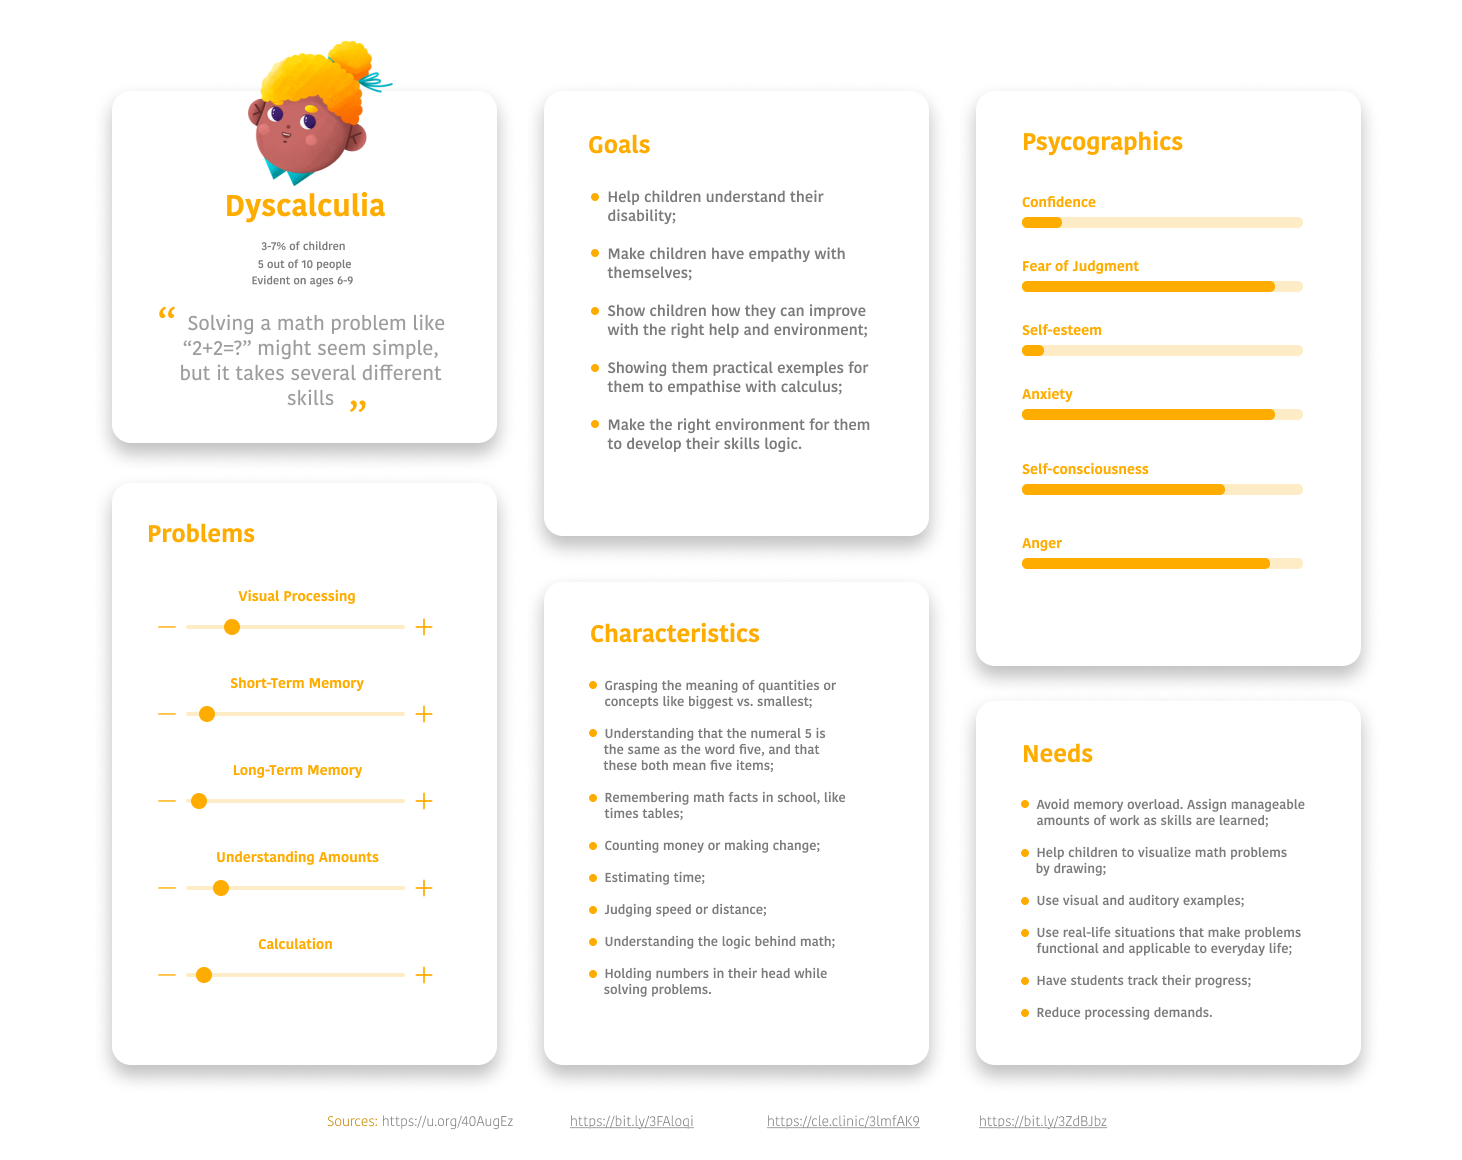
\includegraphics[width=1\linewidth]{Chapters/figma/Discalculia.png}
    \caption{Dyscalculia User Profile}
    \label{fig:dyscalculiaUserProfile}
\end{figure}

\paragraph{Goals}
\begin{itemize}
    \item \textbf{Help children understand their disability}: The mini-games aim to provide children with a clear understanding of Dyscalculia, its impact on their mathematical abilities, and how it does not define their overall intelligence.
    \item \textbf{Foster empathy and self-acceptance}: By creating an environment of empathy and self-acceptance, the mini-games aim to help children develop a positive self-image and reduce negative emotions related to their difficulties with mathematics.
    \item \textbf{Show children how they can improve}: The mini-games should demonstrate to children that with the right help, strategies, and environment, they can improve their mathematical skills and overcome challenges associated with Dyscalculia.
    \item \textbf{Provide practical examples for empathy with calculus}: The mini-games can present practical examples or real-life scenarios to help children develop an empathetic understanding of mathematical concepts and their relevance in everyday life.
    \item \textbf{Create an environment for logical skill development}: The mini-games should provide a supportive and stimulating environment for children to develop their logical and mathematical reasoning abilities.
\end{itemize}

\paragraph{Psycographics}
\begin{itemize}
    \item \textbf{Low confidence}: Children with Dyscalculia often struggle with their mathematical abilities, leading to low confidence in their own skills \cite{understood2024}.
    \item \textbf{Low self-esteem}: Struggles with mathematics can negatively impact self-esteem and self-worth \cite{clevelandclinic2024}.
    \item \textbf{High fear of judgment}: Due to difficulties with math, children may fear being judged or evaluated negatively by peers or teachers \cite{understood2024}.
    \item \textbf{High anxiety}: Children with Dyscalculia may experience anxiety or stress when faced with mathematical tasks or assessments \cite{pmc2024}.
    \item \textbf{High self-consciousness}: Difficulties with mathematics can make children self-conscious about their abilities and performance in academic settings \cite{understood2024}.
    \item \textbf{High anger}: Frustration arising from mathematical challenges can lead to feelings of anger or irritability \cite{clevelandclinic2024}.
\end{itemize}

\paragraph{Problems}
\begin{itemize}
    \item \textbf{Visual processing}: Difficulties in processing and interpreting visual information related to numbers, symbols, and mathematical representations \cite{understood2024}.
    \item \textbf{Short/Long-Term memory}: Challenges in retaining and recalling mathematical facts, formulas, and procedures from both immediate and long-term memory \cite{clevelandclinic2024}.
    \item \textbf{Understanding amounts}: Difficulty grasping the concept of quantity, comparing magnitudes, and understanding number relationships \cite{clevelandclinic2024}.
    \item \textbf{Calculation}: Challenges in performing mathematical calculations, such as addition, subtraction, multiplication, and division \cite{understood2024}.
\end{itemize}

\paragraph{Characteristics}
\begin{itemize}
    \item \textbf{Grasping the meaning of quantities or concepts}: Difficulties in understanding concepts such as big versus small, more versus less, or numerical symbols representing quantities \cite{clevelandclinic2024}.
    \item \textbf{Understanding number-word correspondence}: Struggles in connecting numeral symbols with their corresponding written words and comprehending that they both represent the same quantity \cite{understood2024}.
    \item \textbf{Remembering math facts}: Challenges in recalling and memorizing math facts, such as timestables or basic arithmetic operations \cite{clevelandclinic2024}.
    \item \textbf{Counting money or making change}: Difficulties in accurately counting money, making change, or understanding monetary concepts \cite{clevelandclinic2024}.
    \item \textbf{Estimating time}: Trouble estimating and judging the passage of time accurately \cite{understood2024}.
    \item \textbf{Judging speed or distance}: Challenges in assessing speed, distance, or spatial relationships \cite{pmc2024}.
    \item \textbf{Understanding the logic behind math}: Difficulties in comprehending the underlying logic and reasoning behind mathematical concepts and operations \cite{understood2024}.
    \item \textbf{Holding numbers in their head}: Struggles in retaining and manipulating numbers mentally while solving mathematical problems \cite{clevelandclinic2024}.
\end{itemize}

\paragraph{Needs}
\begin{itemize}
    \item \textbf{Avoiding memory overload}: Assigning manageable amounts of work that align with children's learning abilities and gradually increasing the complexity as skills are learned and mastered \cite{clevelandclinic2024}.
    \item \textbf{Visualizing math problems}: Incorporating visual elements and encouraging children to draw or visualize mathematical problems to enhance understanding and problem-solving \cite{understood2024}.
    \item \textbf{Utilizing visual and auditory examples}: Presenting mathematical concepts and problems through visual and auditory means to address different learning modalities and enhance comprehension \cite{pmc2024}.
    \item \textbf{Real-life applications}: Designing mini-games that incorporate real-life situations and practical examples to demonstrate the functional and applicable aspects of mathematical concepts in everyday life \cite{understood2024}.
    \item \textbf{Tracking progress}: Providing mechanisms for children to track their progress and achievements within the mini-games to foster a sense of accomplishment and motivation.
    \item \textbf{Reducing processing demands}: Implementing strategies and adjustments within the mini-games to reduce cognitive processing demands, such as providing additional time, scaffolding instructions, or offering alternative problem-solving approaches \cite{understood2024}.
\end{itemize}

\subsection{Non-Verbal Learning Disabilities (NVLD)}
Non-verbal learning disabilities (NVLD) are neurodevelopmental conditions that impact a child's ability to understand and interpret non-verbal cues and information. Individuals with NVLD may struggle with social interactions, visual-spatial skills, motor coordination, and executive functioning. To develop interventions tailored to the needs of children with NVLD, it is essential to comprehend their unique user profile. This includes identifying their specific goals, psychographics, problems, characteristics and needs related to non-verbal learning.

\paragraph{Goals}
\begin{itemize}
    \item \textbf{Help children understand their disability}: The mini-games aim to provide children with a comprehensive understanding of NVLD, its impact on their cognitive and social abilities, and how it shapes their unique strengths and challenges.
    \item \textbf{Foster empathy and self-acceptance}: By creating an environment of empathy and self-acceptance, the mini-games aim to help children develop a positive self-image, embrace their differences, and build resilience in the face of challenges.
    \item \textbf{Show children how they can improve}: The mini-games should demonstrate to children that with the right help, strategies, and supportive environment, they can improve their cognitive and social skills and navigate their daily lives more effectively.
    \item \textbf{Explore alternative communication methods}: The mini-games can introduce and explore different modes of communication to help children with NVLD find alternative ways to express themselves effectively.
    \item \textbf{Promote self-acceptance}: The mini-games aim to instill in children the understanding that they do not need to conform to societal expectations and that their unique strengths and perspectives are valuable.
\end{itemize}

\paragraph{Psycographics}
\begin{itemize}
    \item \textbf{High anxiety}: Children with NVLD often experience heightened levels of anxiety related to their difficulties in processing and understanding social and nonverbal cues.
    \item \textbf{High fear of judgment}: Due to challenges in social interactions, children may have a heightened fear of being judged or evaluated negatively by others.
    \item \textbf{Low self-esteem}: Struggles with cognitive and social skills can lead to lower self-esteem and self-worth.
    \item \textbf{High lack of focus}: Difficulties in sustaining attention and focusing on relevant information may be characteristic of children with NVLD.
    \item \textbf{Average self-consciousness}: Children may have an average level of self-consciousness, as they are aware of their challenges but may not fully comprehend the underlying reasons.
    \item \textbf{Low sociability}: Difficulties in social interactions may result in lower levels of social engagement and interaction.
\end{itemize}

\paragraph{Problems}
\begin{itemize}
    \item \textbf{Planning}: Difficulties in organizing and executing sequential tasks or activities effectively.
    \item \textbf{Organization}: Challenges in managing and structuring information, materials, and personal belongings.
    \item \textbf{Problem-solving}: Difficulties in identifying problems, generating solutions, and implementing strategies to resolve them effectively.
    \item \textbf{Recalling visual information}: Challenges in remembering and recalling visual information, such as faces, spatial relationships, or visual details.
    \item \textbf{Picking up social cues}: Difficulty in understanding and interpreting nonverbal cues, gestures, facial expressions, and body language.
\end{itemize}

\paragraph{Characteristics}
\begin{itemize}
    \item \textbf{Remembering information without understanding its significance}: The ability to recall information but struggling to grasp its importance or connect it to broader contexts.
    \item \textbf{Attention to details at the expense of the big picture}: Focusing on specific details while overlooking the overall context or main idea.
    \item \textbf{Physical awkwardness and coordination difficulties}: Exhibiting motor coordination challenges, such as standing too close to others, clumsiness, or poor spatial awareness.
    \item \textbf{Messy handwriting}: Difficulty in producing legible and organized written work.
    \item \textbf{Literal, concrete thinking}: Tendency to think and interpret information in a literal and concrete manner, struggling with abstract or ambiguous concepts.
    \item \textbf{Missing social cues and misreading situations}: Difficulty in understanding and responding to social cues, resulting in misinterpretation of social situations and unawareness of others' reactions.
    \item \textbf{Abruptly changing the subject in conversation}: Shifting topics abruptly during conversations without recognizing the need for smooth transitions.
    \item \textbf{Difficulty adjusting to changes and transitions}: Resistance to changes in routines or environments, finding it challenging to adapt and adjust to new situations.
    \item \textbf{Difficulty organizing thoughts}: Struggles in structuring and organizing thoughts coherently, leading to difficulties in expressing ideas and communicating effectively.
\end{itemize}

\paragraph{Needs}
\begin{itemize}
    \item \textbf{Providing ample warning before transitioning}: Offering clear and advanced notice when transitioning from one activity or task to another, allowing children to mentally prepare and adjust.
    \item \textbf{Making situations more predictable}: Creating predictable and structured environments to reduce anxiety and provide a sense of stability and security.
    \item \textbf{Simplifying visual materials and providing visual aids}: Presenting visual materials in a simplified manner, using visual aids, diagrams, or illustrations to enhance understanding and facilitate information processing.
    \item \textbf{Providing clear, explicit verbal instructions}: Offering precise and unambiguous verbal instructions to ensure clarity and comprehension, helping children to navigate through tasks and activities more effectively.
    \item \textbf{Incorporating movement breaks}: Introducing regular movement breaks within the mini-games to allow children to release energy, improve focus, and enhance cognitive functioning.
    \item \textbf{Providing simple graphic organizers}: Offering graphic organizers such as concept maps or outlines to assist children in organizing their thoughts, fostering structured thinking and facilitating effective communication.
\end{itemize}
\subsection{Dysgraphia}
Dysgraphia is a learning disability that primarily impacts a child's ability to write coherently and express their thoughts through written language. Individuals with dysgraphia may struggle with handwriting, spelling, grammar, and organizing their ideas on paper. In order to develop effective interventions for children with dysgraphia, it is important to understand their unique user profile. This includes identifying their specific goals, psychographics, problems, characteristics, and needs related to written expression and communication.

\begin{figure}[H]
    \centering
    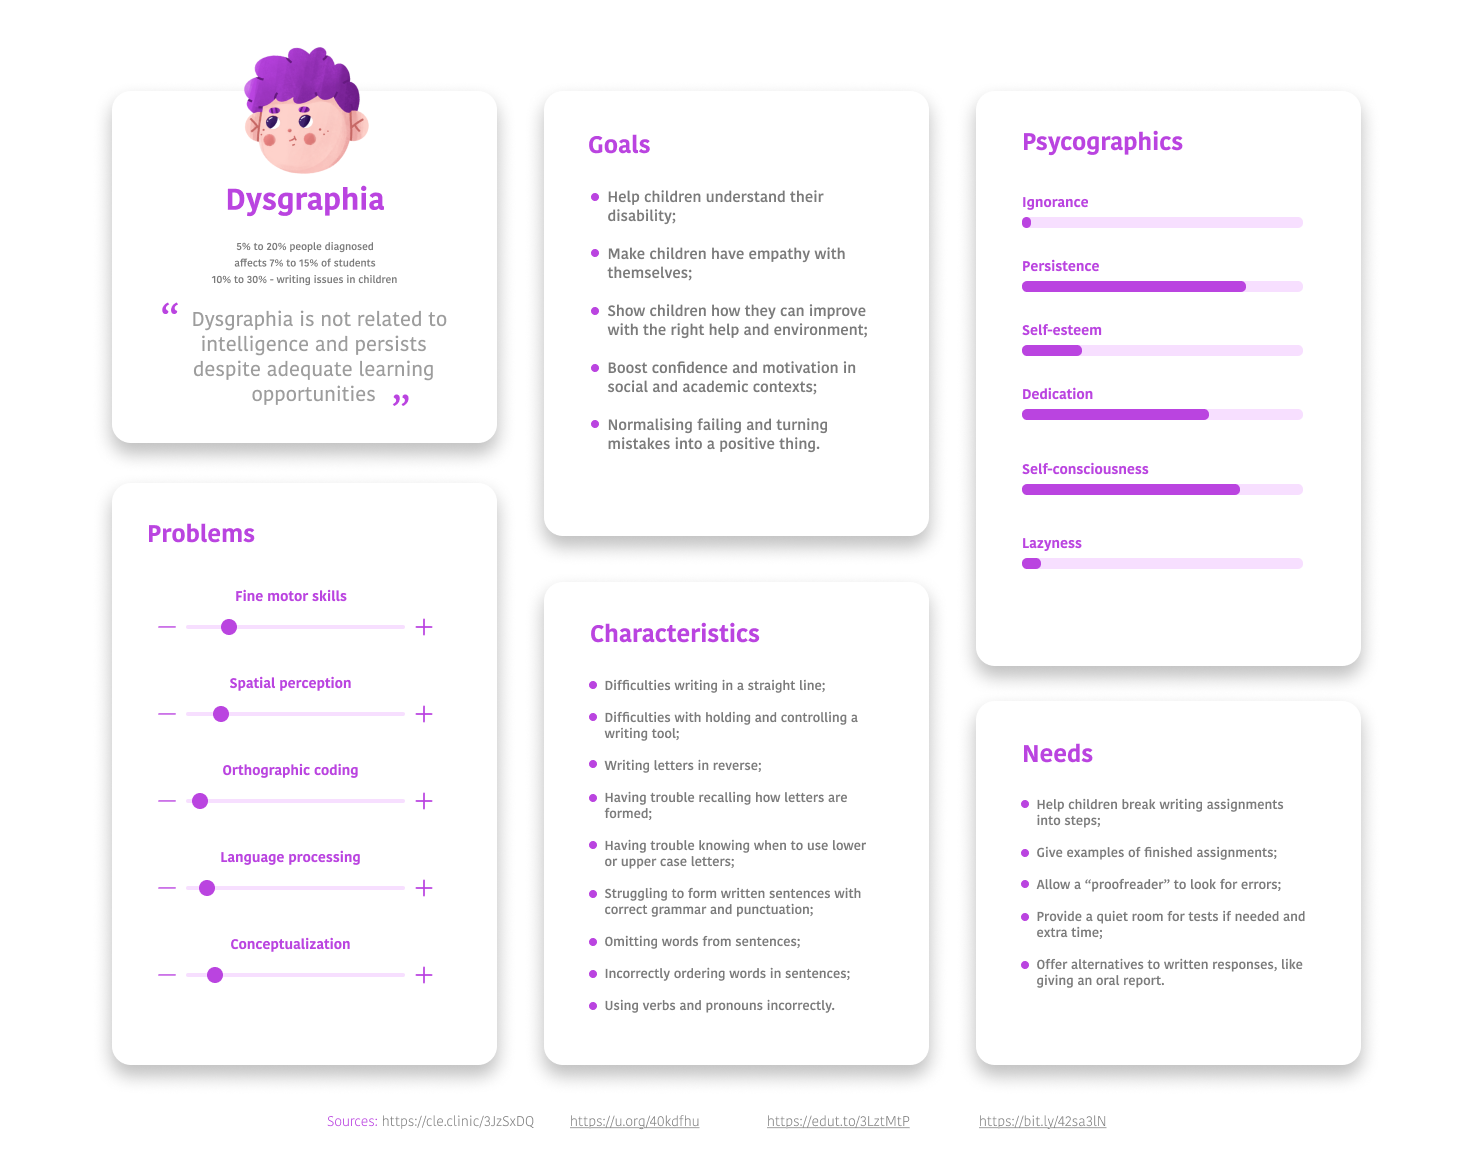
\includegraphics[width=0.8\linewidth]{Chapters/figma/Disgrafia.png}
    \caption{Dysgraphia User Profile}
    \label{fig:disgrafiaUserProfile}
\end{figure}

\paragraph{Goals}
\begin{itemize}
    \item \textbf{Help children understand their disability}: The mini-games aim to provide children with a comprehensive understanding of Dysgraphia, its impact on their writing skills, and the specific challenges they may face.
    \item \textbf{Foster empathy and self-acceptance}: By creating an environment of empathy and self-acceptance, the mini-games aim to help children develop a positive self-image, embrace their unique writing style, and build resilience in the face of writing difficulties.
    \item \textbf{Show children how they can improve}: The mini-games should demonstrate to children that with the right help, strategies, and supportive environment, they can improve their writing skills and overcome specific challenges related to Dysgraphia.
    \item \textbf{Boost confidence and motivation}: The mini-games aim to boost children's confidence in their writing abilities, celebrate their progress and achievements, and enhance their motivation to engage in writing tasks both in social and academic contexts.
    \item \textbf{Normalize failing and turning mistakes into a positive thing}: Creating a positive learning environment within the mini-games that encourages children to view mistakes as opportunities for growth and learning, fostering a growth mindset and resilience.
\end{itemize}

\paragraph{Psychographics}
\begin{itemize}
    \item \textbf{Low ignorance}: Children with Dysgraphia generally have awareness of their writing difficulties and the challenges they face \cite{cleveland_dysgraphia}.
    \item \textbf{High persistence}: Demonstrating persistence and determination in overcoming writing challenges despite all the setbacks.
    \item \textbf{Low self-esteem}: Struggling with writing can negatively impact self-esteem and self-worth \cite{cleveland_dysgraphia}.
    \item \textbf{High dedication}: Displaying a strong commitment and effort in improving writing skills.
    \item \textbf{High self-consciousness}: Being self-conscious about their writing abilities in comparison to their peers.
    \item \textbf{Low laziness}: Exhibiting a proactive and engaged attitude towards writing tasks.
\end{itemize}

\paragraph{Problems}
\begin{itemize}
    \item \textbf{Fine motor skills}: Difficulties in controlling and coordinating fine motor movements required for writing \cite{cleveland_dysgraphia}.
    \item \textbf{Spatial perception}: Challenges in perceiving and reproducing correct spacing, alignment, and proportions of letters and words on a page \cite{cleveland_dysgraphia}.
    \item \textbf{Orthographic coding}: Struggles in remembering and accurately reproducing the correct formation and shape of letters and words \cite{cleveland_dysgraphia}.
    \item \textbf{Language processing}: Difficulties in organizing and expressing thoughts in written form, including grammar, sentence structure, and punctuation \cite{cleveland_dysgraphia}.
    \item \textbf{Conceptualization}: Challenges in generating and organizing ideas coherently and effectively \cite{cleveland_dysgraphia}.
\end{itemize}

\paragraph{Characteristics}
\begin{itemize}
    \item \textbf{Difficulties writing in a straight line}: Struggling to maintain a consistent baseline or alignment while writing \cite{cleveland_dysgraphia}.
    \item \textbf{Difficulties with holding and controlling a writing tool}: Challenges in gripping and controlling the pen or pencil while writing \cite{understood_accommodations}.
    \item \textbf{Writing letters in reverse}: Frequently reversing or inverting letters or numbers \cite{pmc_dysgraphia}.
    \item \textbf{Trouble recalling letter formation}: Difficulty remembering and reproducing the proper formation of letters \cite{edutopia_dysgraphia}.
    \item \textbf{Difficulty with capitalization}: Confusion regarding when to use uppercase or lowercase letters \cite{cleveland_dysgraphia}.
    \item \textbf{Struggling with grammar and punctuation}: Difficulties in using correct grammar, punctuation, and sentence structure \cite{cleveland_dysgraphia}.
    \item \textbf{Omitting or misordering words}: Frequently leaving out words or rearranging them incorrectly within sentences \cite{cleveland_dysgraphia}.
    \item \textbf{Incorrect verb and pronoun usage}: Using verbs and pronouns incorrectly, leading to grammatical errors \cite{cleveland_dysgraphia}.
\end{itemize}

\paragraph{Needs}
\begin{itemize}
    \item \textbf{Breaking writing assignments into steps}: Providing clear and structured instructions, breaking down writing tasks into manageable steps to enhance organization and reduce overwhelm \cite{understood_accommodations}.
    \item \textbf{Providing examples of finished assignments}: Offering visual models and examples of well-organized and properly completed assignments helps understand expectations \cite{understood_accommodations}.
    \item \textbf{Allowing a "proofreader" to look for errors}: Incorporating a feature within the mini-games that allows children to have their written work reviewed by a virtual or real person to identify and correct errors, providing feedback and guidance \cite{understood_accommodations}.
    \item \textbf{Providing a quiet room for tests if needed and extra time}: Recognizing the potential impact of environmental distractions on writing performance and offering a quiet and focused space for assessments, along with appropriate time extensions to accommodate the specific needs of children with Dysgraphia \cite{understood_accommodations}.
    \item \textbf{Offering alternatives to written responses}: Recognizing that writing may pose significant challenges for children with Dysgraphia, the mini-games should provide opportunities for alternative modes of expression, such as giving oral reports or utilizing multimedia formats \cite{understood_accommodations}.
\end{itemize}
\subsection{Auditory Processing Disorder}
Auditory processing disorder (APD) is a neurological condition that affects a child's ability to accurately process and interpret auditory information. Individuals with APD may have difficulty distinguishing sounds, recognizing speech patterns, understanding spoken language, and filtering out background noise. To develop interventions tailored to the needs of children with an auditory processing disorder, it is important to understand their unique user profile. This includes identifying their specific goals, psychographics, problems, characteristics and needs related to auditory processing and communication.

\begin{figure}[H]
    \centering
    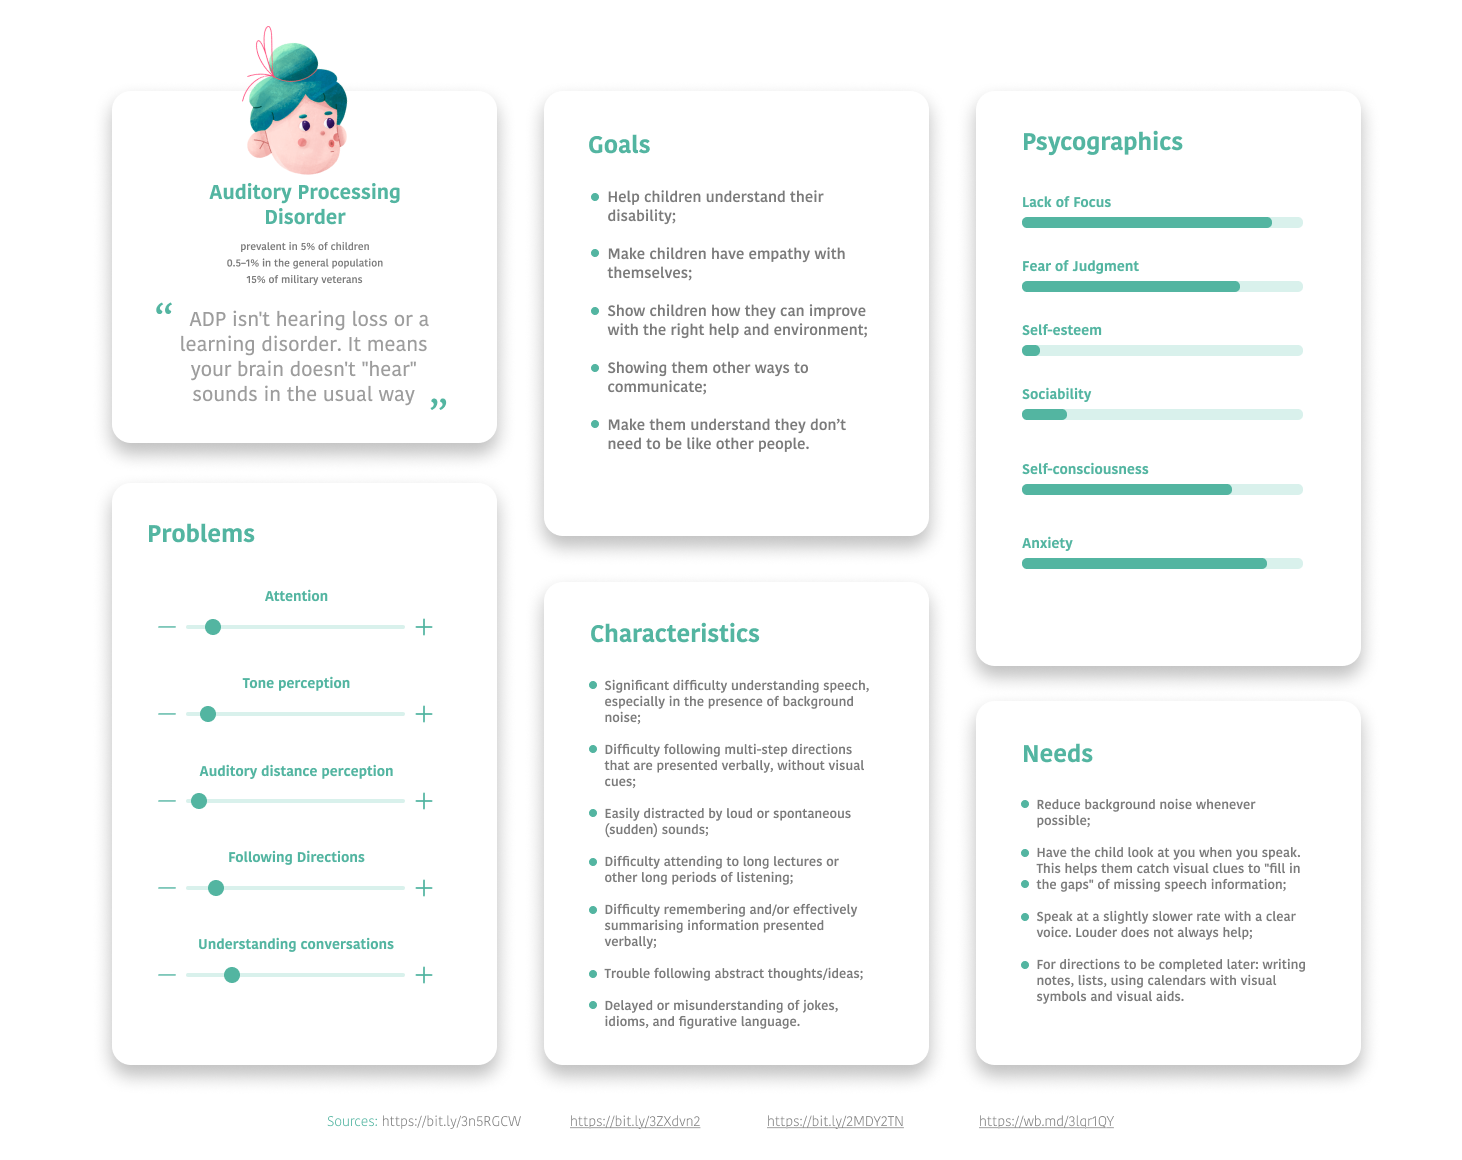
\includegraphics[width=0.8\linewidth]{Chapters/figma/Auditory Processing Disorder.png}
    \caption{Auditory Processing Disorder User Profile}
    \label{fig:APDUserProfile}
\end{figure}

\paragraph{Goals}
\begin{itemize}
    \item \textbf{Help children understand their disability}: The mini-games aim to provide children with a comprehensive understanding of APD, including its impact on their auditory processing skills and the specific challenges they may face in communication and comprehension \cite{Nationwide}.
    \item \textbf{Foster empathy and self-acceptance}: By creating an environment of empathy and self-acceptance, the mini-games aim to help children develop a positive self-image, embrace their unique auditory processing abilities, and build resilience in the face of auditory challenges \cite{KidsHealth}.
    \item \textbf{Show children how they can improve}: The mini-games should demonstrate to children that with the right help, strategies, and supportive environment, they can improve their auditory processing skills and effectively navigate through various listening situations \cite{WebMD}.
    \item \textbf{Provide alternative communication methods}: The mini-games aim to explore and provide children with alternative ways to communicate and comprehend information beyond traditional auditory channels \cite{Nationwide}.
    \item \textbf{Promote self-acceptance}: The mini-games should emphasize that children with APD do not need to compare themselves against others and that their unique auditory processing abilities are valuable in their own right \cite{Nationwide}.
\end{itemize}

\paragraph{Psychographics}
\begin{itemize}
    \item \textbf{High lack of focus}: Difficulty maintaining attention and concentration in auditory tasks due to the challenges in processing auditory information accurately \cite{Nationwide}.
    \item \textbf{High fear of judgment}: Anxiety and fear of being misunderstood or judged by others due to difficulties in comprehending verbal instructions or conversations \cite{KidsHealth}.
    \item \textbf{Low self-esteem}: Struggles with self-worth and confidence, often influenced by difficulties in understanding and responding appropriately to spoken language \cite{WebMD}.
    \item \textbf{Low sociability}: Tendency to withdraw from social interactions due to challenges in understanding and participating in conversations \cite{HearingHealth}.
    \item \textbf{High self-consciousness}: Heightened awareness of their auditory difficulties and how they may be perceived by others \cite{WebMD}.
    \item \textbf{High anxiety}: Experiencing elevated levels of anxiety, particularly in situations involving complex auditory input or noisy environments \cite{Nationwide}.
\end{itemize}

\paragraph{Problems}
\begin{itemize}
    \item \textbf{Attention}: Difficulties in sustaining attention and focus on auditory tasks, particularly in the presence of background noise or competing stimuli \cite{WebMD}.
    \item \textbf{Tone perception}: Challenges in accurately perceiving and interpreting subtle variations in tone and intonation in spoken language, affecting the ability to understand emotions, sarcasm, or subtle nuances in communication \cite{HearingHealth}.
    \item \textbf{Auditory distance perception}: Difficulties in accurately perceiving the distance or location from which sounds originate, which can lead to challenges in localizing sounds or distinguishing relevant auditory cues \cite{Nationwide}.
    \item \textbf{Following directions}: Difficulty comprehending and remembering multi-step directions or instructions that are presented verbally, without visual cues \cite{KidsHealth}.
    \item \textbf{Understanding conversations}: Struggles in processing and comprehending conversations, especially in situations with multiple speakers, fast-paced speech, or complex language structures \cite{Nationwide}.
\end{itemize}

\paragraph{Characteristics}
\begin{itemize}
    \item \textbf{Significant difficulty understanding speech, especially in the presence of background noise}: Struggling to extract relevant information from auditory stimuli, leading to challenges in understanding speech in noisy environments \cite{Nationwide}.
    \item \textbf{Difficulty following multi-step directions without visual cues}: Finding it challenging to retain and follow verbal instructions that involve multiple steps or complex sequencing \cite{KidsHealth}.
    \item \textbf{Easily distracted by loud or spontaneous sounds}: Exhibiting heightened sensitivity to environmental sounds and being easily overwhelmed by unexpected or sudden auditory stimuli \cite{WebMD}.
    \item \textbf{Difficulty attending to long lectures or extended periods of listening}: Struggling to sustain attention and focus during lengthy auditory tasks, such as lectures or extended conversations \cite{Nationwide}.
    \item \textbf{Difficulty remembering and summarizing information presented verbally}: Challenges in retaining and accurately summarizing information presented in spoken form, impacting learning and information processing \cite{WebMD}.
    \item \textbf{Trouble following abstract thoughts and ideas}: Finding it challenging to grasp abstract concepts or complex ideas conveyed through spoken language \cite{HearingHealth}.
    \item \textbf{Delayed or misunderstanding of jokes, idioms, and figurative language}: Difficulties in comprehending and interpreting humor, idiomatic expressions, metaphors, and figurative language, which rely heavily on auditory processing skills \cite{Nationwide}.
\end{itemize}

\paragraph{Needs}
\begin{itemize}
    \item \textbf{Reduce background noise whenever possible}: Creating an auditory environment with minimal distractions and background noise to optimize the child's ability to focus on and process auditory information \cite{KidsHealth}.
    \item \textbf{Encourage visual cues}: Promoting the use of visual cues, such as maintaining eye contact, gestures, facial expressions, and visual aids, to supplement auditory input and enhance comprehension \cite{Nationwide}.
    \item \textbf{Modify speech delivery}: Speaking at a slightly slower rate with a clear and distinct voice, ensuring that instructions and information are presented in a manner that facilitates comprehension for children with APD. Louder speech may not necessarily help and can potentially increase sensory overload \cite{HearingHealth}.
    \item \textbf{Provide visual supports}: Utilizing visual supports, such as written notes, lists, calendars with visual symbols, and visual aids, to reinforce verbal information and assist with memory recall and organization \cite{KidsHealth}.
    \item \textbf{Offer alternative communication methods}: Incorporating alternative modes of communication, such as visual or written responses, within the mini-games to accommodate the needs and preferences of children with APD \cite{Nationwide}.
    \item \textbf{Individualize learning experiences}: Designing mini-games such that can adapt to the unique learning profile of each child with APD, providing personalized challenges and support to foster growth and skill development \cite{Nationwide}.
\end{itemize}


\subsection{Visual Motor Deficit}
Visual motor deficit, also known as visual-motor integration difficulty, refers to a condition that impacts a child's ability to coordinate visual perception with motor skills. Individuals with visual motor deficits may experience challenges in tasks requiring hand-eye coordination, spatial awareness, and fine motor control. To develop interventions tailored to the needs of children with visual motor deficits, it is important to understand their unique user profile. This includes identifying their specific goals, psychographics, problems, characteristics, and needs related to visual-motor integration and motor coordination.

\begin{figure}[H]
    \centering
    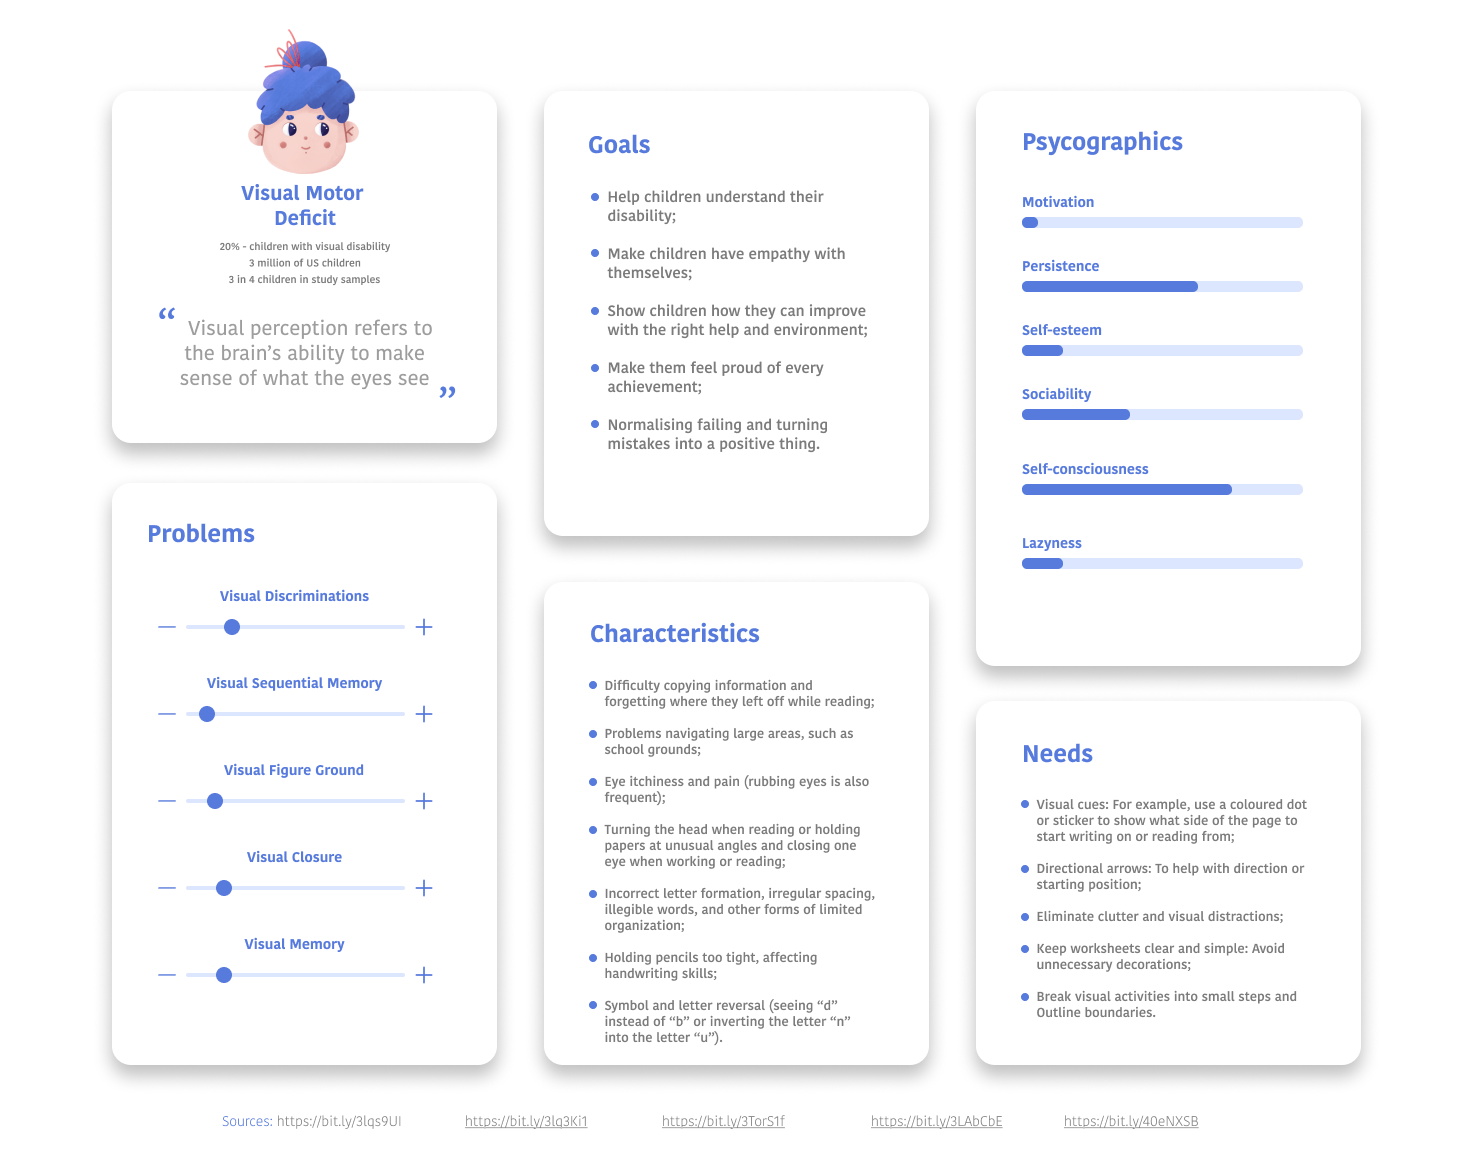
\includegraphics[width=0.8\linewidth]{Chapters/figma/Visual Motor Deficit.png}
    \caption{Visual Motor Deficit User Profile}
    \label{fig:VMDUserProfile}
\end{figure}

\paragraph{Goals}
\begin{itemize}
    \item Helping children understand their disability and fostering self-empathy.
    \item Demonstrating how improvement is achievable with appropriate support and an enabling environment.
    \item Cultivating a sense of pride in every achievement, no matter how small.
    \item Promoting a positive mindset towards failure, viewing mistakes as opportunities for growth.
\end{itemize}

\paragraph{Psycographics}
\begin{itemize}
    \item Low motivation and self-esteem due to persistent challenges \cite{ChildDevelopment}.
    \item High levels of persistence, showing determination to overcome difficulties \cite{Speechify}.
    \item Average sociability, seeking opportunities for interaction with peers \cite{PorterAcademy}.
    \item Heightened self-consciousness about their motor skills \cite{Speechify}.
    \item Low levels of laziness, indicating a willingness to invest effort in learning and development \cite{PorterAcademy}.
\end{itemize}

\paragraph{Problems}
\begin{itemize}
    \item \textbf{Visual discriminations}: Difficulty distinguishing and recognizing visual details accurately \cite{ChildDevelopment}.
    \item \textbf{Visual sequential memory}: Struggles in remembering and reproducing visual sequences in the correct order \cite{PorterAcademy}.
    \item \textbf{Visual figure-ground}: Difficulty differentiating foreground from background in visual stimuli \cite{ScienceDaily}.
    \item \textbf{Visual closure}: Challenges in perceiving complete images or letters when parts are missing \cite{Speechify}.
    \item \textbf{Visual memory}: Difficulty retaining and recalling visual information accurately \cite{PorterAcademy}.
\end{itemize}

\paragraph{Characteristics}
\begin{itemize}
    \item Difficulty copying information accurately and maintaining their place while reading \cite{Speechify}.
    \item Challenges in navigating large areas and perceiving spatial relationships \cite{PorterAcademy}.
    \item Frequent eye itchiness and pain, leading to rubbing of the eyes \cite{ChildDevelopment}.
    \item Unusual head movements or holding papers at atypical angles while reading or working \cite{Speechify}.
    \item Poor letter formation, irregular spacing, and illegible handwriting \cite{PorterAcademy}.
    \item Excessive grip pressure on pencils, impacting handwriting skills \cite{ScienceDaily}.
    \item Reversal of symbols and letters, such as mistaking ''d'' for ''b'' or inverting the letter ''n'' into ''u'' \cite{ChildDevelopment}.
\end{itemize}

\paragraph{Needs}
\begin{itemize}
    \item \textbf{Visual cues}: Incorporating visual aids, such as colored dots or stickers, to signal the starting point for writing or reading \cite{PorterAcademy}.
    \item \textbf{Directional arrows}: Providing clear visual cues to assist with direction and starting positions \cite{Speechify}.
    \item \textbf{Minimizing clutter and distractions}: Creating organized and uncluttered learning environments to enhance focus and concentration \cite{ChildDevelopment}.
    \item \textbf{Simplifying worksheets}: Presenting worksheets with clear, straightforward designs and avoiding unnecessary decorations \cite{Speechify}.
    \item \textbf{Breaking activities into small steps}: Breaking down visual tasks into manageable steps to facilitate understanding and completion \cite{ScienceDaily}.
    \item \textbf{Outlining boundaries}: Using visual cues, such as borders or highlighting, to delineate boundaries within worksheets or assignments \cite{PorterAcademy}.
\end{itemize}


\section{Some examples}
\label{sec:gamesforld}
	% (Apresentar exemplos de trabalho relacionado)
	% (Procurar por jogos idênticos que tratem o mesmo problema)

Before the development of the games themselves, we should first look into some other existing solutions. This will allow for some advantages as we can analyse each one, knowing which characteristics are better suited for the mini-games being developed in this thesis.
As we are developing different games targeted for different age groups and disabilities, we will have to group our research for games that aim to help for each \gls{ld}. This way, we can capture some characteristics for each game and it will be easier when developing each mini-game from scratch.
Next, we'll present some of the games found that can be useful for the research.

\newpage
\subsection*{Fast ForWord} 

Fast ForWord\cite{fastforword} is a game that helps children will \textbf{dyslexia} and \textbf{Language Processing Disorder} to improve their phonological awareness, auditory processing and skills. It uses adaptive technology to provide individualized feedback and instruction.
Fast  ForWord is based on the neuroscience principles of neuroplasticity, the ability of the brain to change and adapt in response to stimulation and learning. It consists of two phases: cognitive and reading. The cognitive phase works on skill gaps and building fundamentals, such as processing, working memory, attention, and sequencing. The reading phase trains reading fluency and comprehension as well as vocabulary, grammar, and syntax. It has 9 programs in total each with 5-7 exercises that target different aspects of learning and reading. Each program is designed for different age groups and levels of difficulty.
According to a meta-analysis of over 300 efficacy and research studies, Fast ForWord users achieved an average gain of 2 years in reading skills in about 6 months. \cite{gemlearningFastFor}
One of the games consists of listening to a story and then answering questions and following instructions. This improves skills in listening comprehension and builds familiarity with English language conventions. Figure \ref{fig:fastforword} shows the aspect of this game in specific.

\begin{figure}[!h]
    \centering
    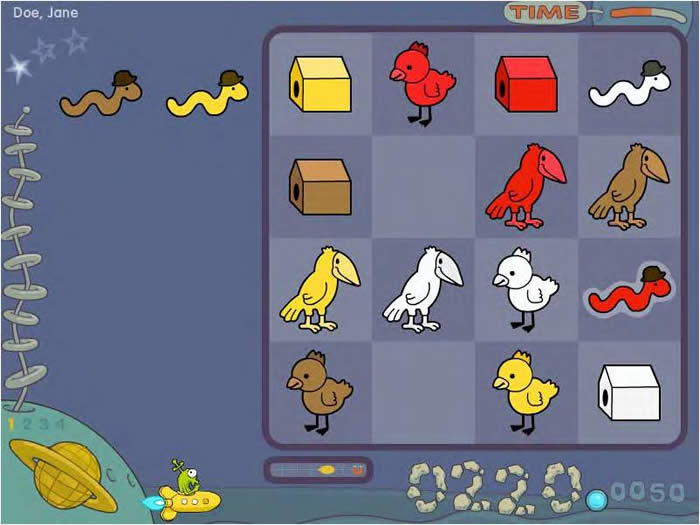
\includegraphics[width=0.8\linewidth]{Chapters/related_work_img/FastForWord_Cosmic_Reader.jpg}
    \caption{Fast ForWord - Cosmic Reader}
    \label{fig:fastforword}
\end{figure}
% https://www.gemmlearning.com/programs/fast-forword/

% https://www.apa.org/topics/learning-memory/dyslexia-video-games
% https://www.scilearn.com/ - Game Site

% https://www.apa.org/topics/learning-memory/dyslexia-video-games
% https://www.unicef.org/parenting/child-care/10-playful-educational-activities-children-disabilities
% https://www.parentcircle.com/games-and-activities-for-special-needs-and-autistic-children/article
% https://www.commonsensemedia.org/articles/5-ways-video-games-can-help-kids-with-disabilities
% https://parentingpod.com/dyslexia-activities/


\subsection*{NumberShire} 

NumberShire \cite{numbershire} is an internet-based game that aims at educationg children with intense focus on critical whole number concepts and skills for students. It is made for all students, but specially for those with difficulties in mathematics. This directly impacts children with dyscalculia and other math-related \glspl{ld}.

It was developed with support from the U.S Department of Education. It achieved great results in several controlled trials, with students having significant gains in their math skills, against students with typical math support.

The game is composed of mathematical concepts in a story-based, fantasy setting. Players complete quests by solving math problems tailored to their specific skill level. Through this narrative, children learn foundational math concepts such as addition, subtraction, and number sense. The game provides immediate feedback and rewards progress, creating a motivational framework that encourages practice.

Figure \ref{fig:numberShire} details the visual representation of the gameplay.

\begin{figure}[!h]
    \centering
    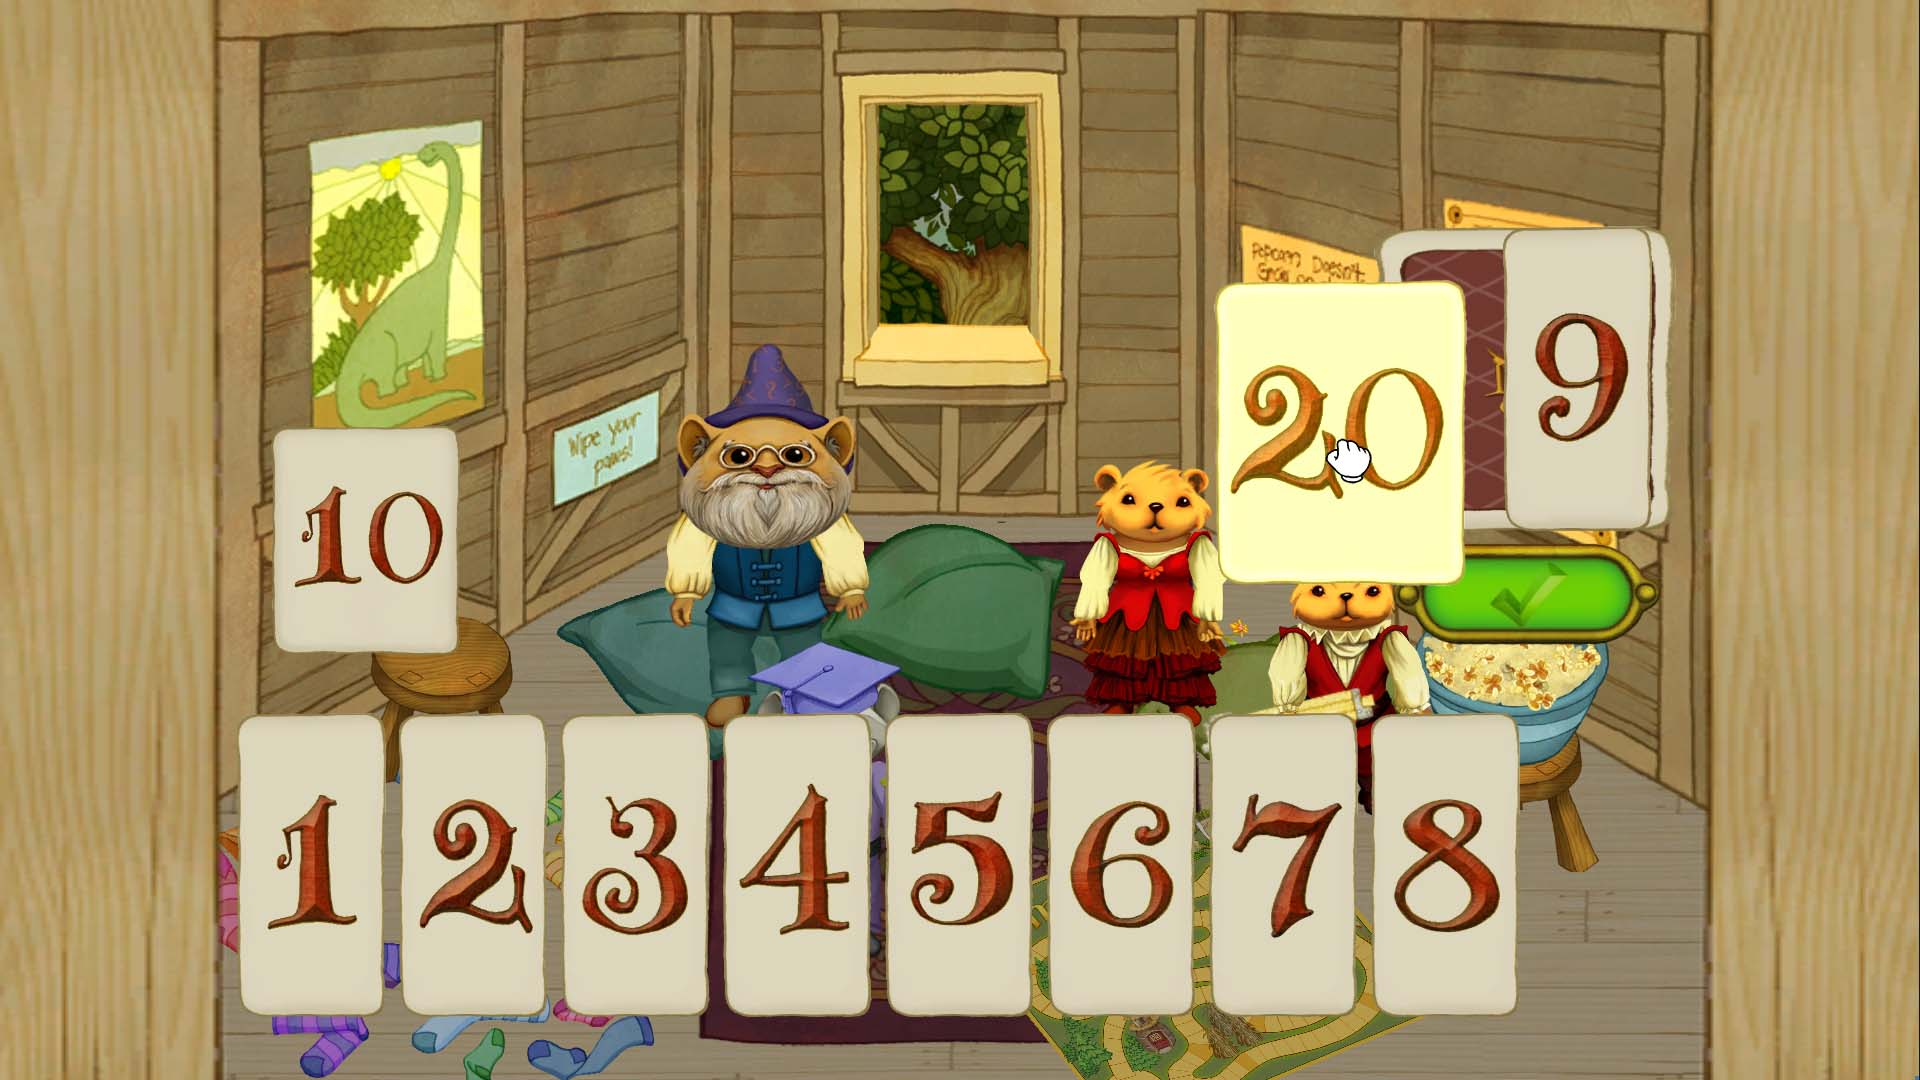
\includegraphics[width=0.8\linewidth]{Chapters/related_work_img/NumberShire_gameplay02.jpg}
    \caption{NumberShire - Gameplay}
    \label{fig:numberShire}
\end{figure}


\subsection*{GraphoGame}
% The best results have been found in children aged 5 to 8, although - in practice - it is useful for struggling readers of any age and children as young as 4. 

GraphoGame \cite{graphogamesoftware} is an educational game developed by a Finnish company. The game is meant to be played on touch-screen devices such as smartphones or tablets.

In the game, players create their own avatar and start to train from the most fundamental skills. It starts with letter recognizing, connecting letters with sounds. After that, children start to do letter combinations, combining sounds into syllabes and, lastly they move to challenging syllabes and complicated words. This sequence is know as the synthetic approach to reading instruction.

The game adapts in real-time to the child’s performance, offering more challenging or simplified content based on their success rate. This adaptive nature is particularly beneficial for children with dyslexia, as it allows for targeted practice on challenging areas without overwhelming the learner. It utilizes a simple interface, having all instructions spoken aloud. GraphoGame is designed for children aged from six to eight years old. However it can be useful for readers of any age \cite{ronimus2019supporting}.

Figure \ref{fig:graphogame} displays one of the challenges inside the game.

\begin{figure}[H]
    \centering
    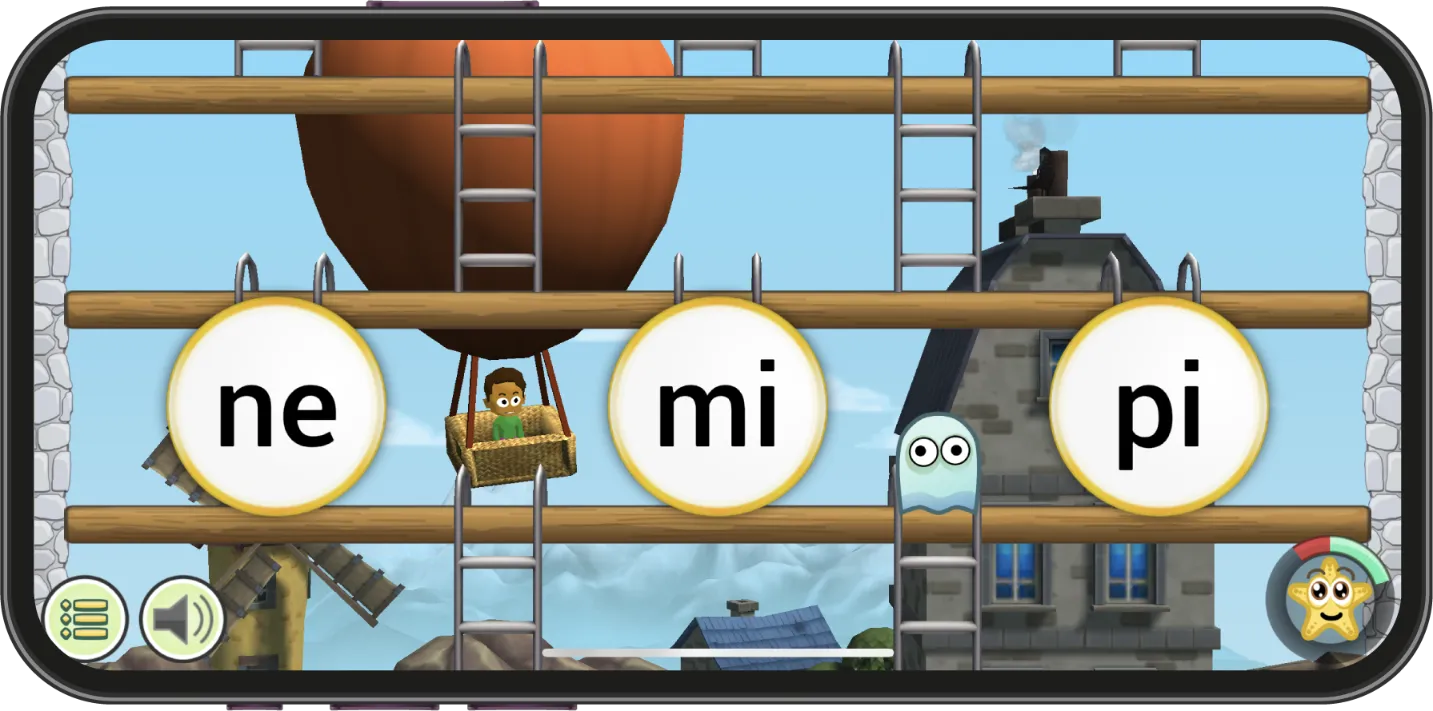
\includegraphics[width=0.8\linewidth]{Chapters/related_work_img/graphogamegameplay.png}
    \caption{GraphoGame - Gameplay}
    \label{fig:graphogame}
\end{figure}



% (No início do capítulo, colocar um resumo sobre o mesmo, indicando 
% o conteúdo de cada secção)


% This chapter describes how to use the  \texttt{LaTeX} style thesis{}. This style file is a major rewrite from the most of Universities, which was in turn adapted from a style file from the FCT-UNL (not official version).  We aimed at providing an improved visual layout and, simultaneously, a \emph{very easy to use} template (aka, a  \texttt{LaTeX} template for dummies). 

% \noindent%
% \fbox{%
% \begin{minipage}{\linewidth}
% 	The first main rule you must know is that \textbf{you must} specify the encoding of your text files. A simple \emph{rule of thumb} is: if you are using Windows add 'latin1' to the list of package options; if you are using other systems, such as Linux or Mac OSx, add 'utf8' to the list of package options.
% \end{minipage}%
% }
% % section introduction (end)

% % ====================
% % = Folder Structure =
% % ====================
% \section{Folder Structure} % (fold)
% \label{sec:folder_structure}

% The template file for writing dissertations in  \texttt{LaTeX} is organized into a main directory, a set of files and sub-directories:
% \begin{enumerate}
% 	\item[ThesisISEL] This is the main directory and includes:
% 	\begin{enumerate}
% 		\item \textbf{Logo} Directory with Faculty logos;
% 		\item \textbf{sty} Directory will all sty files that help in formatting document;
% 		\item \textbf{Chapters} Directory where to put user files (text and figures);
% 		\begin{enumerate}
% 		\item \textbf{scripts} Directory with useful bash scripts, e.g., for cleaning all temporary files;
% 		\item \textbf{img} Directory with all images of your thesis;
% 		\end{enumerate}
% 		\item \textbf{alpha-pt.bst} A file with bibliography names in portuguese, e.g., 'Relatório Técnico' e 'Tese de Mestrado' instead of 'Technical Report' and 'Master Thesis'. This file is used automatically if Portuguese is selected as the main language (see below);
% 		\item \textbf{defaults.tex} A file with the main default values for the package (institution name, faculty's logo, degree name and similars);
% 		\item \textbf{personaldataofthesis.tex} A file with the main default values for the package (identification of report as well as the author and juries);
% 		\item \textbf{template.tex} The main file. You should run  \texttt{LaTeX} in this one. Please refrain from changing the file content outside of the well defined area;
% 		\item \textbf{bibliography.bib} The bib file. An easy way to find to import citation into \texttt{bibtex} is select option \texttt{Show links to import citation into
% Bib\-Tex} in \href{http://scholar.google.pt/scholar_settings?hl=en&as_sdt=0,5}{\texttt{Scholar google settings}}.
% 		\item \textbf{thesisisel.cls} The  \texttt{LaTeX} class file for the thesis{} style. Currently, some of the defaults are stored here instead of \verb!defaults.tex!. This file should not be changed, unless you're ready to play with fire! :)
% 	\end{enumerate}
% \end{enumerate}

% Again, we would like to recall that all the user \texttt{LaTeX} files should be stored in the \verb!ThesisISEL! directory, and all the images in \verb!ThesisISEL/Chapters/img! directory.\todo[inline]{Yet another note!}
% % section folder_structure (end)

% % ===================
% % = Package options =
% % ===================
% \section{Package Options} % (fold)
% \label{sec:package_options}

% The thesis{} style includes the following options, that must be included in the options list in the \verb!\documentclass[options]{thesisisel}! line at the top of the \texttt{template.tex} file.

% The list below aggregates related options in a single item. For each list, the default value is prefixed with a *.

% \subsection{Language Related Options} % (fold)
% \label{sub:language_related_options}

% You must choose the main language for the document. The available options are:

% \begin{enumerate}
% 	\item \textbf{*pt} --- The text is written in Portuguese (with a small abstract in English).
% 	\item \textbf{en} --- The text is written in English (with a small abstract in Portuguese).
% \end{enumerate}

% The language option affects:
% \begin{itemize}
% 	\item \textbf{The order of the summaries.} At first the abstract in the main language and then in the foreign language. This means that if your main language for the document in english, you will see first the abstract (in english) and then the 'resumo' (in portuguese). If you switch the main language for the document, it will also automatically switch the order of the summaries.
% 	\item \textbf{The names for document sectioning.} E.g., 'Chapter' vs.\ 'Capítulo', 'Table of Contents' vs.\ 'Índice', 'Figure' vs.\ 'Figura', etc.
% 	\item \textbf{The type of documents in the bibliography.} E.g., 'Technical Report' vs.\ 'Relatório Técnico', 'MSc Thesis' vs.\ 'Tese de Mestrado', etc.
% \end{itemize} 

% No mater which language you chose, you will always have the appropriate hyphenation rules according to the language at that point. You always get portuguese hyphenation rules in the 'Resumo', english hyphenation rules in the 'Abstract', and then the main language hyphenation rules for the rest of the document. If you need to force hyphenation write inside of \verb!\hyphenation{}! the hyphenated word, e.g. \\
% \verb!\hyphenation{op-ti-cal net-works}!.
% % section package_options (end)

% \subsection{Class of Text} % (fold)
% \label{sub:class_of_text}

% You must choose the class of text for the document. The available options are:

% \begin{enumerate}
% 	\item \textbf{bsc} --- BSc graduation report.
% 	\item \textbf{prepmsc} --- Preparation of MSc dissertation. This is a preliminary report graduate students at ISEL/IPL must prepare to conclude the first semester of the two-semesters MSc work. The files specified by 
% 	\begin{inparaenum}
% 	\item \verb!\dedicatoryfile! and 
% 	\item \verb!\acknowledgmentsfile! 
% 	\end{inparaenum}
% 	are ignored, even if present, for this class of document.
% 	\item \textbf{msc} --- MSc dissertation.
% \end{enumerate}
% %% subsection class_of_text (end)
% %
% %% ============
% %% = Printing =
% %% ============
% \subsection{Printing} % (fold)
% \label{sub:printing}

% You must choose how your document will be printed. The available options are:

% \begin{enumerate}
% \item \textbf{oneside} --- Single side page printing, and
% \item \textbf{*twoside} --- Double sided page printing.
% \end{enumerate}

% The article 50th, of Decree-Law No. 115/2013, requires the deposit of a digital copy of doctoral thesis and master's dissertations in a repository that is part of the RCAAP  repository\footnote{Repositórios Científicos de Acesso Aberto de Portugal}, \url{https://www.rcaap.pt}.  This deposit aims to preserve scientific work, as well as providing Open Access to scientific production is not restricted object or embargo.

% For the reason explained above, we include the option to format your thesis in a way that presents well on screen and/or on paper.   But always remember that your work will be stored in the RCAAP portal in electronic format.
% % subsection printing (end)

% The available options are:

% \begin{enumerate}
% \item \textbf{onpaper} --- Format your thesis in a way that presents on paper or,
% \item \textbf{*onscreen} --- on screen.
% \end{enumerate}

% % =============
% % = Font Size =
% % =============
% \subsection{Font Size} % (fold)
% \label{ssec:font_size}

% You must select the encoding for your text. The available options are:
% \begin{enumerate}
% 	\item \textbf{11pt} --- Eleven (11) points font size.
% 	\item \textbf{*12pt} --- Twelve (12) points font size. You should really stick to 12pt\ldots
% \end{enumerate}
% % subsection font_size (end)

% % =================
% % = Text encoding =
% % =================
% \subsection{Text Encoding} % (fold)
% \label{ssec:text_encoding}

% You must choose the font size for your document. The available options are:
% \begin{enumerate}
% 	\item \textbf{latin1} --- Use Latin-1 (\href{http://en.wikipedia.org/wiki/ISO/IEC_8859-1}{ISO 8859-1}) encoding.  Most probably you should use this option if you use Windows;
% 	\item \textbf{utf8} --- Use \href{http://en.wikipedia.org/wiki/UTF-8}{UTF8} encoding.    Most probably you should use this option if you are not using Windows.
% \end{enumerate}
% % subsection font_size (end)

% % ============
% % = Examples =
% % ============
% \subsection{Examples} % (fold)
% \label{ssec:examples}

% Let's have a look at a couple of examples:

% \begin{itemize}
% 	\item BSc graduation report, in portuguese, with 11pt size and to be printed one sided (I wonder why one would do this!)\\
% 	\verb!\documentclass[bsc,pt,11pt,oneside,latin1]{thesisisel}!
% 	\item Preparation of MSc thesis, in portuguese, with 12pt size and to be printed one sided (I wonder why one would do this!). Note that, \verb!pt! is declared by default, so it can be omitted: \\
% 	\verb!\documentclass[prepmsc,12pt,oneside,latin1]{thesisisel}!
% 	\item MSc dissertation, in english, with 12pt size and to be printed double sided on screen. Note that, \verb!twoside! and \verb!12pt! are declared by default, so it can be omitted: \\
% 	\verb!\documentclass[msc,en,utf8,onscreen]{thesisisel}!
% \end{itemize}


% The present document is defined according to the following settings:
% \begin{Verbatim}[breaklines=true, breakanywhere=true]
% \documentclass[msc,pt,twoside,12pt,a4paper,utf8,onscreen,hyperref=true,listof=totoc] {thesisisel}
% \end{Verbatim}

% % subsection examples (end)
	
% \section{How to Write Using \texttt{LaTeX}} % (fold)
% \label{sec:how_to_write_using_latex}

% Please have a look at Chapter~\ref{cha:a_short_latex_tutorial_with_examples}, where you may find many examples of \href{http://tobi.oetiker.ch/lshort/lshort.pdf}{\texttt{LaTeX}} constructs, such as sectioning, inserting figures and tables, writing equations, theorems and algorithms, exhibit code listings, etc.

% %% section how_to_write_using_latex (end)
